\clearpage\nobalance\normalsize
\section*{Author Notes}
\subsection*{Acknowledgements}
\textbf{Course instructor: Professor Luyao Zhang.} The project uses Python, NumPy, Matplotlib, nbclient, Gradio, and the instructor-provided COMSCI/ECON 206 PS2 Overleaf and poster structures. All computational inputs are stylized/synthetic; no empirical participant dataset was used. OpenAI Codex assisted implementation, debugging, literature-search support, verification, restructuring, and drafting under human review. Appendix~D documents Feiyu Li's dated review of a superseded project version without presenting it as peer validation of the current model. Yiqiao Liu remains responsible for the proposal, citations, computations, and errors.

\subsection*{Team and individual contributions}
\noindent\textbf{Joint contribution (single-member Team FP10; 126 words).} The integrated contribution is to turn a low-altitude traffic privacy tension into an auditable chain across three disciplines. The project makes commercial-disclosure granularity a Bayesian action, compares equilibrium with a realized-type welfare benchmark, and tests whether reciprocal access to enhanced non-safety services can change incentives without conditioning mandatory safety information. Exhaustive computation exposes both the benchmark improvement and failure regions rather than treating one favorable parameter point as a theorem. A bounded priority-slot comparison separates upstream information sharing from downstream scarcity allocation. The behavioral decision environment then converts the rational prediction, privacy and fairness mechanisms, and a misunderstanding alternative into inspectable Solo and Peer Play prompts. Linked code, notebooks, outputs, and evidence-status labels make the claim reproducible while reserving empirical and policy conclusions for future tests.

\noindent\textbf{Yiqiao Liu; author order: 1.} Liu decided to separate mandatory safety information from voluntary commercial disclosure and to report CCAR as a candidate, not an optimum. The concrete outputs are the model and tests in \texttt{src/} and \texttt{tests/}, notebooks in \texttt{notebooks/}, behavioral artifacts in \texttt{hf\_space/} and \texttt{hf\_static/}, and this paper. Verification comprises exhaustive equilibrium/first-best calculations, seeded simulations, browser checks, hosted Colab Run-all confirmations, and 65 automated passes. The model outputs feed the decision artifact and paper figures. For final submission, Liu is responsible for accurately documenting review scope, rerunning affected checks, finalizing the poster, and approving every claim change.

\bibliographystyle{ACM-Reference-Format}
\bibliography{references}

\appendix
\section{Technical details and reproducibility}
\label{app:technical}
Nature independently draws $c_A,c_B\in\{1,1.6\}$, each with probability $1/2$, and publicly reveals $d$. Each operator observes only its own type, then chooses simultaneously. A pure strategy is $s_i:\{L,H\}\rightarrow\{M,P,F\}$. Against $s_j$, type $t_i$ evaluates
\[
EU_i(a\mid t_i,s_j,d)=\sum_{t_j}\Pr(t_j)u_i(a,s_j(t_j);t_i,d).
\]
A profile is a pure BNE iff every prescribed action attains this maximum. The first best separately maximizes $W=u_A+u_B$ over nine profiles for every $(c_A,c_B,d)$ and then averages with the prior; it assumes observed types and need not be implementable.

\begin{table}[H]
\caption{Normalized benchmark inputs.}
\centering\small
\begin{tabular}{@{}ll@{}}\toprule
Primitive & Value \\\midrule
Actions & $M,P,F$; $x=(0,1,2)$; $k=(0,1,2.5)$ \\
Types/prior & $c=(1,1.6)$; $(0.5,0.5)$ independent \\
Congestion & $d=(0.3,0.6,1.0)$ public \\
Technology & $B=7.5$; $\lambda=0.5$ \\
CCAR & $\alpha_M=0.7$ at Medium/High; others $1$ \\
Auction & 4 bidders; $U[0,10]$; 10,000 rounds \\
Seeds & benchmark 206; bid-noise stress 1206 \\
\bottomrule\end{tabular}
\end{table}

\noindent\textbf{Language-independent pseudocode.}
\begin{enumerate}
\item For every congestion state, enumerate each player's mappings from types to actions.
\item For every strategy pair and own type, average each action's payoff over rival types; retain pairs in which all prescribed actions are best responses.
\item For every realized type pair, enumerate action profiles and retain all welfare maximizers; average equilibrium and first-best welfare under the prior.
\item Replace enhanced-access factors according to CCAR, recompute equilibrium utility, and evaluate underlying welfare without counting denied access as a benefit.
\item Repeat over confidentiality, Full-cost, access, and congestion grids; record multiplicity and failure diagnostics.
\item For the allocation extension, compare first eligible allocation with highest bid/second payment, then repeat seeded draws and bid-noise perturbations.
\end{enumerate}

\begin{table*}[t]
\caption{Interim expected utility of each action against the benchmark equilibrium rival strategy. The rival strategy and chosen action are ordered by own type $(L,H)$.}
\label{tab:eu}
\centering
\small
\begin{tabular}{@{}llcrrrl@{}}
\toprule
Congestion & Own type & Rival strategy & $EU(M)$ & $EU(P)$ & $EU(F)$ & Equilibrium choice \\
\midrule
Low & $L$ & $(M,M)$ & \textbf{0.000} & -0.115 & -1.078 & $M$ \\
Low & $H$ & $(M,M)$ & \textbf{0.000} & -0.715 & -2.578 & $M$ \\
Medium & $L$ & $(P,M)$ & 0.885 & \textbf{1.308} & 0.670 & $P$ \\
Medium & $H$ & $(P,M)$ & \textbf{0.885} & 0.708 & -0.830 & $M$ \\
High & $L$ & $(P,P)$ & 2.951 & \textbf{3.741} & 3.327 & $P$ \\
High & $H$ & $(P,P)$ & 2.951 & \textbf{3.141} & 1.827 & $P$ \\
\bottomrule
\end{tabular}
\end{table*}


\begin{table}[H]
\caption{Validated equilibrium and welfare outputs.}
\centering\small
\begin{tabular}{@{}lrrrr@{}}\toprule
$d$ & BNE $(L,H)$ & $W_{BNE}$ & $W_{FB}$ & Gap \\\midrule
Low & $(M,M)$ & 0.000 & 0.639 & 0.639 \\
Medium & $(P,M)$ & 2.193 & 3.139 & 0.946 \\
High & $(P,P)$ & 6.882 & 7.385 & 0.503 \\
\bottomrule\end{tabular}
\end{table}

\begin{figure*}[t]
\centering
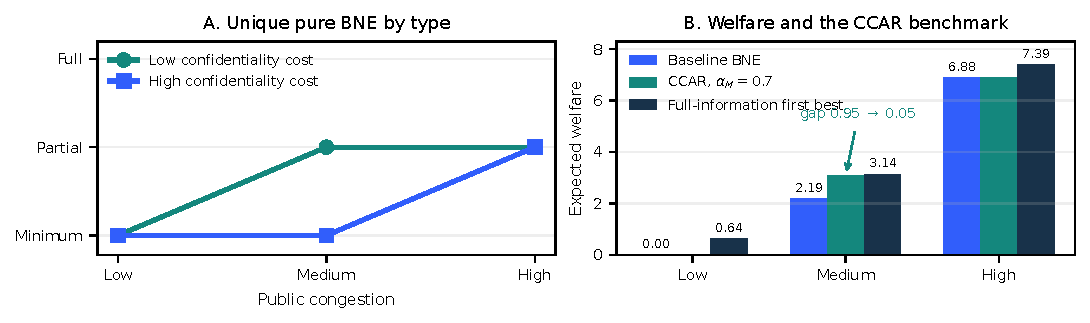
\includegraphics[width=\textwidth]{figures/main_results.pdf}
\caption{Tracked computational outputs: type-contingent BNE actions (left) and underlying expected welfare (right). At Medium, CCAR changes $(P,M)$ to $(P,P)$ and reduces the gap from $0.946$ to $0.050$; Low and High coincide with baseline.}
\Description{Equilibrium actions rise with congestion. Grouped bars compare baseline BNE, CCAR welfare, and full-information first best.}
\label{fig:results}
\end{figure*}

\subsection{Mechanism sensitivity, actual outputs, and known failures}
CCAR scales only the recipient's enhanced non-safety coordination value: at Medium/High, $\alpha(M)=\alpha_M$ and $\alpha(P)=\alpha(F)=1$; at Low all equal one. At $\alpha_M=0.7$, Medium BNE is $(P,P)$, underlying welfare is $3.089$, and the gap is $0.050$. The Medium access sweep gives $(P,P)$ through $0.70$, two asymmetric equilibria at $0.75$, and baseline $(P,M)$ from $0.80$. The 760-cell grid counts 401 no-effect, 334 robust-improvement, 18 excessive-disclosure, 3 increased-gap, 66 multiple-BNE, and 0 no-pure-BNE cases; diagnostics overlap and are not probabilities. Lower Full exposure costs can induce Full disclosure. These results show parameter dependence, discontinuous equilibrium-set transitions, and the need for an equilibrium selection rule in multiplicity regions.

\subsection{Reproduction record}
Inputs are the stylized primitives above; baseline is unrestricted enhanced access, comparisons are CCAR, FCFS, and truthful second price; metrics are equilibrium actions, welfare/gap, multiplicity, failure flags, revenue, and efficiency. Checkpoint \CurrentCommit{} was fresh-run with Python 3.13.7, NumPy 2.3.5, Matplotlib 3.10.8, nbclient 0.10.2, and Gradio 6.29.0. The automated suite reports \textbf{65 passed, 0 failed}: 27 computational, 6 notebook-portability, 17 Gradio behavioral, and 15 static/export checks. Both hosted \ColabOne{} and \ColabTwo{} were manually confirmed by the student to complete Run all. Deterministic notebooks are \path{notebooks/01_strategic_disclosure_game.ipynb} and \path{notebooks/02_priority_slot_allocation.ipynb}; shortest reproduction is open each Colab and Run all. Tracked CSV/PNG/SVG outputs are under \texttt{outputs/}. The behavioral version is the \SpaceRepo{} tied to exported provenance data. The validated editable poster is \texttt{\seqsplit{poster/PS2-FP10-Yiqiao-A0-Poster.pptx}}.

Limitations are two operators, two independent types, three actions, exogenous congestion, pure equilibria, normalized uncalibrated parameters, no implementation-cost model, and no representative behavioral sample. The first best observes types; CCAR omits enforcement/administration; auction welfare omits urgency, wealth, and interdependent values.

\subsection*{Open Science Statement}
The \PublicRepo{}, \ColabOne{}, \ColabTwo{}, and \SpaceRepo{} expose code, stylized/synthetic inputs, dependency files, checkpoint \CurrentCommit{}, and actual outputs. No private dataset, secret, or external LLM is required at runtime. Run-all notebooks reproduce equilibrium, welfare, CCAR, sensitivity, and auction outputs. The repository license and institutional deployment terms govern reuse; absence of empirical calibration and behavioral sampling limits external validity.

\subsection*{Statement of Contribution to the UN's SDGs}
No demonstrated SDG contribution is claimed at proposal stage. Prospective relevance to safe, inclusive infrastructure requires target-level justification, an access and delay baseline, stakeholder-defined safety/confidentiality outcomes, distributional and unintended-effect audits, a field comparison, and a public correction or suspension rule.

\subsection{AI-use disclosure}
\textbf{Tool/model and date.} OpenAI Codex, a GPT-5-based coding agent, was used on 2 October 2026. \textbf{Purpose.} Assistance covered implementation, debugging, test design, literature-search support, browser and reproducibility checks, document restructuring, and drafting/editing. \textbf{Significant prompt categories.} Prompts asked for Bayesian-game enumeration, welfare/CCAR validation, allocation simulation, behavioral-interface construction, deployment, artifact parity, evidence auditing, and official-template compliance. \textbf{Accepted suggestions.} Exhaustive-strategy verification, explicit separation of mechanism utility from underlying welfare, bounded auction language, machine-testable evidence labels, and the official A--F reorganization were retained after inspection. \textbf{Rejected or qualified suggestions.} Any absolute novelty, universal mechanism superiority, empirical behavioral effect, invented review, invented contact/session metadata, and completed-poster implication were rejected or qualified. \textbf{Human revisions.} Yiqiao Liu chose the question, model boundary, parameters, welfare interpretation, CCAR framing, evidence boundary, and final wording. \textbf{Verification and responsibility.} Claims were checked against tracked CSVs, code, cited primary sources, 65 tests, notebook runs, browser checks, PDF rendering, and clean-package compilation. Liu accepts responsibility for every claim, citation, computation, and submission decision.

\section{Cumulative Intellectual Development}
\begin{table}[H]
\caption{Auditable development record; topic continuity is not implied.}
\centering\scriptsize
\begin{tabularx}{\columnwidth}{@{}p{1.6cm}p{2.0cm}YY@{}}\toprule
Earlier claim & Dated evidence/feedback & Revision & Intellectual consequence \\\midrule
The earlier ``Stay or Switch?'' version studied AI memory portability. & Feiyu Li's 28 Sept. 2026 review raised equilibrium multiplicity and the need for behavioral verification of switching. & The research direction later changed substantially to low-altitude strategic disclosure; the old comments were not relabeled as review of the new model. & The new project retained the methodological demand for robustness, explicit incentives, behavioral evidence boundaries, and reproducibility. \\
A favorable mechanism point could motivate a proposal. & 2 Oct. 2026 computational checkpoint exposed parameter sensitivity and multiplicity. & Added CCAR sweeps and a 760-cell failure grid. & The claim became conditional and falsifiable, not universal. \\
The rational model could stand alone. & 2 Oct. 2026 behavioral-artifact checkpoint made alternative explanations inspectable. & Added Solo/Peer Play, benchmark reveal, CCAR second choice, and reflection. & Future evidence can separate preference/framing from misunderstanding. \\
Notebook results were locally reproducible. & 2 Oct. 2026 portability checkpoint \texttt{ffa4836} and manual hosted Run-all confirmation. & Added self-bootstrapping Colab paths and reconciled test counts. & Reproduction now has a public, auditable shortest path. \\
\bottomrule\end{tabularx}
\end{table}

\clearpage\onecolumn
\section{Open-source and three-lens inspiration}
\begin{table}[H]
\caption{Sources and tools actually used.}
\centering\scriptsize
\begin{tabularx}{\textwidth}{@{}p{1.6cm}p{2.5cm}p{1.6cm}p{1.4cm}YYY@{}}\toprule
Tool/source & Official URL & License & Version/date & Capability & Limitation & Design consequence \\\midrule
Python & \url{https://www.python.org/} & PSF & 3.13.7 & Reproducible implementation/tests & Environment-dependent & Locked dependencies and tests \\
NumPy & \url{https://numpy.org/} & BSD-3-Clause & 2.3.5 & Arrays and seeded simulation & Floating-point arithmetic & Explicit tolerances/seeds \\
Matplotlib & \url{https://matplotlib.org/} & PSF-based & 3.10.8 & Static result figures & No inference by itself & Figures read tracked outputs \\
nbclient & \url{https://nbclient.readthedocs.io/} & BSD-3-Clause & 0.10.2 & Notebook execution & Hosted runtime differs & Added portability tests/Colab bootstrap \\
Gradio & \url{https://www.gradio.app/} & Apache-2.0 & 6.29.0 & Decision-interface prototype & Not a sampling frame & Evidence labeled exploratory \\
acmart & \url{https://www.acm.org/publications/proceedings-template} & LPPL & 2.20, 2026-08-16 & Course paper typesetting & Layout, not evidence & Official template organization retained \\
Course template & Instructor-provided repository & Course-provided & Autumn 2026 & Required topology/checklist & Contains prompts, not results & Five sections and Appendices A--F \\
\bottomrule\end{tabularx}
\end{table}

\noindent\textbf{Three lenses.} Game theory changes the project by requiring complete type-contingent strategies and interim mutual best responses, predicting $M/P/F$. Social choice adds the realized-type first best, welfare gap, disclosure-burden ties, and an explicit efficiency/fairness comparison. Mechanism design changes the feasible institution: CCAR makes enhanced non-safety access reciprocal and demands equilibrium and welfare robustness checks while preserving a mandatory safety floor.

\noindent\textbf{Week 4 literature stress test.} Chin et al. challenge the congestion/coordination and limited-information dimensions \cite{chin2022efficient,chin2023traffic}; Maheshwari et al. challenge privacy-preserving coordination \cite{maheshwari2025privacy}; Su et al. and Vickrey challenge scarcity allocation \cite{su2024vertiport,vickrey1961counterspeculation}; Raith challenges endogenous strategic information sharing \cite{raith1996general}. The surviving gap is only their intersection: type-contingent disclosure granularity with private commercial-confidentiality cost and congestion-dependent coordination value, followed by a separately bounded allocation stage.
\begin{center}
\captionsetup{hypcap=false}
\captionof{table}{Closest-literature comparison. Entries summarize substantive overlap; definitions need not be identical.}
\label{tab:literature}
\centering
\scriptsize
\begin{tabularx}{\textwidth}{@{}p{0.17\textwidth}ccccccY@{}}
\toprule
Study & AAM & Privacy / limited info & Endogenous disclosure & Private conf. cost & Congestion-value link & Auction / allocation & Relationship \\
\midrule
Chin et al. (2022) \cite{chin2022efficient} & Yes & No & No & No & Yes & No & Centralized efficiency/fairness benchmark with dynamic demand. \\
Chin et al. (2023) \cite{chin2023traffic} & Yes & Yes & No & No & Yes & Yes & Decentralized protocol minimizes shared trajectory detail and includes optional cost-aware prioritization. \\
Maheshwari et al. (2025) \cite{maheshwari2025privacy} & Yes & Yes & No & No & Yes & Yes & Privacy-preserving capacity allocation with private vehicle valuations and anonymous prices. \\
Su et al. (2024) \cite{su2024vertiport} & Yes & Indirect & No & No & Yes & Yes & Incentive-compatible vertiport reservation with heterogeneous private valuations. \\
Raith (1996) \cite{raith1996general} & No & Strategic info & Yes & No & No & No & General oligopoly incentives to share private demand/cost information. \\
This project & Yes & Yes & Yes & Yes & Yes & Downstream & Disclosure granularity is a type-contingent action; CCAR and auction remain bounded extensions. \\
\bottomrule
\end{tabularx}
\end{center}


\section{Review response and revision record}
\begingroup\footnotesize
\subsection{Peer review of superseded PS2 version}
On 28 September 2026, Feiyu Li (FP3 member 1) reviewed FP10's earlier AI memory-portability project, ``Stay or Switch?'' The sheet identifies Session B and Yiqiao Liu. It recognized parameter/model cross-checking and passing-test/reproducibility work; raised the priority concern that equilibrium multiplicity weakened benchmark welfare conclusions; asked whether real users switch when portability exists; suggested participant switching data from the Hugging Face Space; and recommended \textbf{Revise}. \textbf{This review does not constitute direct peer validation of the final low-altitude drone-disclosure model.}

\subsection{Methodological lessons retained after the research-direction change}
The topic changed substantially, so the comments were not treated as direct revisions to the new model. Three lessons carry over: (1) the multiplicity concern reinforced explicit multiple-equilibrium reporting and caution against universalizing one equilibrium; the CCAR grid reports 66 multiple-pure-BNE cells; (2) the request for observed switching reinforced the boundary between computational prediction and behavioral evidence; the Hugging Face artifact is an exploratory classroom exercise, not representative evidence about real drone operators; and (3) the emphasis on checks appears in 65 passed and 0 failed, public GitHub, two runnable Colabs, a public Space, and claim/source audits. These carryovers do not imply endorsement of the current model.

\subsection{Current-version review status}
No topic-specific peer review of the final low-altitude drone-disclosure version was available before final submission. The only received peer review concerned the superseded memory-portability version and is therefore used solely as part of the methodological-development record. Earlier-version peer review: \textbf{RECEIVED AND DOCUMENTED}. Current-version topic-specific peer review: \textbf{NOT AVAILABLE BEFORE FINAL SUBMISSION}. No current-version reviewer question or Keep/Revise/Investigate decision is invented.
\endgroup

\clearpage\onecolumn
\section{Structured abstract and cumulative proposal map}
\label{app:abstract}
\begin{table}[H]
\caption{Official eight-row structured abstract.}
\label{tab:abstract-map}
\renewcommand{\arraystretch}{1.16}
\begin{tabularx}{\textwidth}{@{}p{0.27\textwidth}Y@{}}\toprule
\textbf{Proposal element} & \textbf{Current statement / change} \\\midrule
Background & Urban low-altitude operators gain coordination value from flight-intent sharing but may expose commercially sensitive demand; safety disclosure remains mandatory. \\
Motivation and application & Capacity-constrained drone-delivery corridors require both useful coordination and legitimate allocation of residual commercial priority among stakeholders with different safety, access, and confidentiality concerns. \\
Three connected questions & Economics asks how congestion and private costs shape BNE versus first best; computation maps welfare and CCAR robustness; behavior tests privacy, reciprocity/fairness, competitive concern, and misunderstanding. \\
Method and model assumptions & Two-player simultaneous Bayesian game, independent binary types, three disclosure actions, public congestion, exhaustive pure-BNE/first-best enumeration, parameter sweeps, bounded auction, and exploratory decision artifact. \\
Results or expected results & Actual: BNE $(M,M),(P,M),(P,P)$ and gaps $0.639,0.946,0.503$; benchmark CCAR lowers Medium gap to $0.050$. Planned: discriminating behavioral and pilot tests; no population effect claimed. \\
Intellectual merits & Integrates endogenous disclosure, auditable welfare comparison, mechanism failure mapping, and behaviorally distinguishable assumptions without claiming absolute novelty. \\
Practical impacts & Prospective benefit is avoided delay; risks include confidentiality, unequal access, over-disclosure, and misspecification. Adoption needs calibration, safety/distributional review, audit, appeal, and suspension rules. \\
Feedback received and revision made & One review concerned a superseded memory-portability version. Because the project later changed direction, it was not treated as direct validation of the current model. Its lessons motivated stronger multiplicity reporting, clearer behavioral-evidence boundaries, and reproducibility checks. No topic-specific review of the final drone-disclosure version was available before final submission. \\
\bottomrule\end{tabularx}
\end{table}

\noindent\textbf{Cumulative proposal map.} The earlier AI memory-portability framing was replaced, rather than cosmetically continued, by low-altitude strategic interaction. Its September 28 review remains scoped to that superseded topic, while its methodological demand for robustness, behavioral verification boundaries, and reproducibility carries forward. The Bayesian model feeds verified computation; computation feeds the Solo/Peer Play benchmark and Figure~\ref{fig:results}; the bounded auction and real-world governance record state where the analogy and evidence stop. Actual results, planned tests, and the unavailability of current-topic feedback before final submission remain separately labeled.

\clearpage\twocolumn
\section{PS2 extension record: auction, linked artifacts, poster, and symposium}
\subsection{Auction laboratory record}
\label{app:auction}
The scarce resource is one short-window priority slot in a congested corridor. Participants are eligible non-emergency commercial operators; emergency/public-safety flights remain outside payment. Benchmark values/signals are independent private values; reports are sealed bids. In the deterministic case, $v_A=8,v_B=5,v_C=3,v_D=2$ and FCFS order is $B,C,A,D$. The planned/rational Vickrey bid equals value; truthful bidding is weakly dominant. FCFS allocates to the first eligible request and stops. Second price allocates to the highest bid, breaks ties by ID, charges the second-highest bid, and stops.

Actual computation: FCFS gives $B$ value $5$, efficiency $0.625$; truthful second price gives $A$, payment/revenue $5$, winner utility $3$, efficiency $1$. Over 10,000 seed-206 rounds, mean FCFS/auction efficiencies are $0.622308/1.000000$, allocated values $4.96856/7.99983$, and second-price revenue $5.99207$. The behavioral stress test uses mean-one lognormal bid noise (seed 1206): efficiency/misallocation is $0.989514/0.1393$ at $\sigma=.1$, $0.956564/0.2783$ at $.25$, $0.904572/0.4124$ at $.5$, and $0.826281/0.5467$ at $1$. These are simulations, not classroom observations. Interpretation: truthful IPV allocation is an efficiency benchmark, not a blanket policy ranking; urgency, ability to pay, common values, and institutional legitimacy break the analogy.

\subsection{Linked-artifact parity}
\begin{tabularx}{\columnwidth}{@{}p{1.65cm}Y@{}}\toprule
\textbf{Artifact}&\textbf{Required parity check}\\\midrule
GitHub&Same payoff, parameters, BNE, welfare, CCAR, auction outputs, checkpoint \texttt{ffa4836}, runnable paths, and limits.\newline\PublicRepo \\
Hugging Face&Same $M/P/F$ setting, benchmark reveal, CCAR, behavioral alternatives, no-sample boundary, and no PII/telemetry.\newline\SpaceRepo \\
A0 poster&Uses the same questions, results, case, limitations, instructor, acknowledgements, and links. Validated editable file: \texttt{\seqsplit{PS2-FP10-Yiqiao-A0-Poster.pptx}}. \\
\bottomrule\end{tabularx}

\subsection{Symposium and practical-impact record}
Symposium session: \SymposiumSession. The superseded-version review is documented in Appendix~D. Current-topic review: \textbf{NOT AVAILABLE BEFORE FINAL SUBMISSION}. No current-version presentation question or Keep/Revise/Investigate decision is recorded or invented. The concrete case is commercial drone-delivery operators sharing capacity-constrained urban low-altitude corridors. Stakeholders are operators, the traffic-management authority, customers, nearby/public stakeholders, and emergency/public-safety users. Proposed benefit is coordination and avoided delay. Risks are confidentiality loss, unequal access, over-disclosure, and misspecified incentives. Missing evidence includes field/pilot calibration, operational latency, confidentiality valuation, safety review, and distributional effects. Correction requires auditable rules, a safety-information floor, appeal/review, and parameter revision or suspension when welfare or access diagnostics fail.
